% This is a simple sample document.  For more complicated documents take a look in the exercise tab. Note that everything that comes after a % symbol is treated as comment and ignored when the code is compiled.
% !TEX program = xelatex

\documentclass{ctexart} % \documentclass{} is the first command in any LaTeX code.  It is used to define what kind of document you are creating such as an article or a book, and begins the document preamble

\usepackage{amsmath} % \usepackage is a command that allows you to add functionality to your LaTeX code
\usepackage{amssymb}
\usepackage{booktabs}
\usepackage{graphicx}
\usepackage{float}
\usepackage{caption}
\usepackage{subcaption}
\usepackage[T1]{fontenc}
\usepackage{lmodern}  % scalable CM/Latin Modern fonts
\usepackage{fix-cm}   % allow arbitrary scaling (reduces size substitution warnings)
\title{Simple Sample} % Sets article title
\author{My Name} % Sets authors name
\date{\today} % Sets date for date compiled

% The preamble ends with the command \begin{document}
\begin{document} % All begin commands must be paired with an end command somewhere
\maketitle % creates title using information in preamble (title, author, date)
LaTeX 完整章节(不含任何代码)。请直接复制到 CUMCM 模板中使用。
\section{精确模型:多光束干涉与Airy公式}

在问题一中,我们建立了基于双光束干涉的理想模型。然而,在实际物理情景中,光波会在外延层的上下两个界面(空气-外延层界面、外延层-衬底界面)之间发生多次反射和透射,形成多光束干涉,如图2所示。这种效应在特定条件下会变得十分显著,从而影响测量精度。本节旨在建立一个更精确的多光束干涉模型。

我们考虑一个厚度为 $d$、折射率为 $n$ 的均匀外延层。设空气-外延层界面的振幅反射系数和透射系数分别为 $r_{01}$ 和 $t_{01}$,外延层-衬底界面的振幅反射系数为 $r_{12}$。当一束平面波入射时,总的反射光是无穷多束反射子波的相干叠加。

第1束反射光的复振幅为 $E_1 = r_{01}E_0$。后续的反射光束需要进出外延层,相邻光束间的光程差为 $2nd\cos\varphi$,对应的相位差为:
$$
    \delta = \frac{2\pi}{\lambda} (2nd\cos\varphi) = 4\pi n d \nu \cos\varphi
$$
其中 $\nu$ 是波数,$\varphi$ 是在外延层内的折射角。

通过对所有出射的反射光束的复振幅进行等比数列求和,并利用斯托克斯关系式进行化简,可以得到总的振幅反射系数 $\rho = E_R / E_0$ 为:
$$
    \rho = \frac{r_{01} + r_{12} e^{-i\delta}}{1 + r_{01} r_{12} e^{-i\delta}}
$$
我们最终测量的物理量是反射率 $R$,即反射光强与入射光强之比,它等于振幅反射系数的模的平方 $R = |\rho|^2$。经过推导,总反射率 $R$ 可以表示为著名的 \textbf{Airy 公式}:
$$
    R(\delta) = \frac{(r_{01} + r_{12})^2 - 4r_{01}r_{12}\sin^2(\delta/2)}{(1 + r_{01}r_{12})^2 - 4r_{01}r_{12}\sin^2(\delta/2)}
$$
为了更直观地理解干涉条纹的形状,上式通常被写为:
$$
    R = \frac{F \sin^2(\delta/2)}{1 + F \sin^2(\delta/2)}
$$
其中,$F$ 被称为 \textbf{精细度系数 (Coefficient of Finesse)},它由界面的强度反射率 $R_1 = r_{01}^2$ 和 $R_2 = r_{12}^2$ 决定:
$$
    F = \frac{4\sqrt{R_1 R_2}}{(1-\sqrt{R_1 R_2})^2}
$$
精细度系数 $F$ 衡量了干涉条纹的锐利程度。当 $F$ 值较小(即界面反射率较低)时,Airy公式的行为近似于 $\sin^2$ 函数,对应于双光束干涉的宽缓条纹。当 $F$ 值较大(即界面反射率较高)时,干涉峰会变得非常尖锐,谷底平坦宽阔,这是多光束干涉的典型特征。这一模型为我们分析附件3和4中硅晶片的光谱,以及修正碳化硅光谱的计算精度提供了坚实的理论基础。

\subsection{多光束干涉产生的必要条件}
基于光波在薄膜内多次反射的物理图像(图2),要产生显著的多光束干涉效应,而非退化为双光束干涉,需满足以下必要条件:

\begin{itemize}
    \item \textbf{核心条件一:界面高反射率}。外延层-衬底界面的反射率 $R_{\text{int}}$(近似为 $R_{ns} = \left( \frac{n - n_s}{n + n_s} \right)^2$)必须足够高。若 $R_{\text{int}}$ 过低(经验值 $R_{\text{int}} \lesssim 0.1$),则二次以上反射光束的强度将呈指数级衰减($\propto R_{\text{int}}^k$),其叠加贡献可忽略不计,系统退化为双光束干涉模型。反之,高 $R_{\text{int}}$ 值会显著提高干涉条纹的锐度(对比度),其影响可由 \textbf{精细度系数} $F = \frac{4R_{\text{int}}}{(1-R_{\text{int}})^2}$ 量化,$F$ 值越大,条纹越尖锐。

    \item \textbf{核心条件二:薄膜低吸收率}。外延层材料对入射光波长的吸收系数 $\alpha$ 必须足够小,以确保光在多次往返传播过程中的强度衰减不明显。其定量条件为 $\alpha \cdot 2d \ll 1$。若吸收过强,高次反射光束的振幅将因损耗而急剧减弱($\propto e^{-\alpha \cdot 2k d}$),同样导致多光束效应被抑制。
\end{itemize}

\noindent 此外,以下两个辅助条件对维持清晰、稳定的干涉图样至关重要:

\begin{itemize}
    \item \textbf{辅助条件一:界面平行与膜厚均匀}。外延层上下界面应近似平行,且膜厚 $d$ 及折射率 $n$ 在光斑区域内均匀一致。否则,不同位置产生的干涉条纹会发生叠加平均,导致整体条纹对比度下降甚至消失。

    \item \textbf{辅助条件二:入射光相干性}。入射光需具有良好的时间与空间相干性,其相干长度 $L_c$ 应大于光在薄膜内的最大往返光程(即 $L_c \geq 2nd\cos\varphi$)。对于本题所用的傅里叶变换红外光谱(FTIR)技术,虽采用宽带光源,但在窄带干涉滤波下,仍可在特定波数处满足相干性要求,形成稳定的干涉条纹。
\end{itemize}

\noindent 在本问题中,硅(Si)与碳化硅(SiC)材料属性的差异直接决定了多光束干涉效应的显著性:
\begin{itemize}
    \item 对于\textbf{硅晶片}(附件3、4),外延层与衬底虽同为硅材料,但因掺杂浓度不同导致折射率存在差异,其界面反射率 $R_{\text{int}}^{\text{Si}}$ 较高(通常可达$0.2$以上),易满足核心条件一,故光谱呈现出尖锐的干涉峰(高精细度),多光束干涉效应显著。
    \item 对于\textbf{碳化硅晶片}(附件1、2),外延层与衬底界面的折射率差较小,导致 $R_{\text{int}}^{\text{SiC}}$ 较低(约$0.05$量级),更接近双光束干涉条件,其干涉条纹较为平滑。但其吸收系数 $\alpha$ 在红外波段同样较低,满足核心条件二。
\end{itemize}

\subsection{硅外延层厚度的计算与分析}

本节旨在根据多光束干涉理论,分析附件3和附件4中硅(Si)晶圆片的光谱特性,建立数学模型并设计算法,最终确定其外延层厚度。

\subsubsection{模型与算法选择}

在上一节中,我们通过定性分析确认了硅晶圆片光谱呈现出典型的多光束干涉特征。其核心数学描述是Airy公式。理论上,可以通过非线性最小二乘法对整个光谱进行Airy公式拟合来求解厚度 $d$。然而,该方法存在以下挑战:
\begin{itemize}
    \item \textbf{参数耦合与色散效应}:Airy公式中的折射率 $n$ 并非一个常数,而是随波数 $\nu$ 变化的函数(即色散效应)。这使得全局拟合的参数众多、高度耦合,极易陷入局部最优或不收敛,在竞赛有限时间内难以获得稳定可靠的结果。
    \item \textbf{计算复杂度高}:非线性拟合过程计算量大,对初始参数的猜测非常敏感,调试过程耗时。
\end{itemize}

考虑到上述因素,并注意到一个关键事实:\textbf{无论是双光束干涉还是多光束干涉,干涉极大值(峰值)的位置均遵循相同的物理规律}。即干涉峰位满足:
$$
    2nd\cos\varphi = m\lambda \quad (m \text{为整数})
$$
这使得基于峰间距 $\overline{\Delta\nu}$ 的算法具有极好的普适性和稳健性。因此,我们选择该方法作为计算硅外延层厚度的主要算法,其不仅计算高效、结果稳定,而且已在问题二中得到验证。

\subsubsection{数学模型与算法实现}

我们的模型基于干涉极大值条件。对于相邻的两个干涉峰,其波数分别为 $\nu_k$ 和 $\nu_{k+1}$,对应的干涉级次相差1。由此可得:
$$
    2nd\cos\varphi \cdot (\nu_{k+1} - \nu_k) = 1
$$
假设在整个测量波段内,硅的折射率 $n$ 近似为常数,则峰间距 $\Delta\nu = \nu_{k+1} - \nu_k$ 也应为常数。厚度 $d$ 的计算公式为:
$$
    d (\mu\text{m}) = \frac{10^4}{2n\cos\varphi \cdot \overline{\Delta\nu}}
$$
其中,$\varphi$ 为外延层内的折射角,由斯涅尔定律 $\sin\theta = n\sin\varphi$ 决定。

算法实现步骤如下:
\begin{enumerate}
    \item \textbf{参数确定}:通过查阅文献\cite{Green2008Silicon},我们确定硅(Si)在近红外波段的折射率 $n_{\text{Si}}$ 近似为常数 $3.42$。
    \item \textbf{数据读取与寻峰}:读取附件3和附件4的数据,使用\texttt{scipy.signal.find\_peaks}函数进行自动寻峰。由于硅光谱的峰形尖锐,我们设置了\texttt{prominence}参数以有效识别主峰,避免噪声干扰。
    \item \textbf{峰间距计算与稳健估计}:计算所有相邻峰位之间的波数差 $\Delta\nu_k$。为消除潜在的异常值影响,我们采用IQR(四分位距)准则对 $\Delta\nu_k$ 集合进行筛选,仅保留位于 $[Q_1 - 1.5 \cdot \text{IQR}, Q_3 + 1.5 \cdot \text{IQR}]$ 区间内的数据点,然后计算其算术平均值,得到稳健的平均峰间距 $\overline{\Delta\nu}$。
    \item \textbf{厚度计算}:将 $n_{\text{Si}}$、入射角 $\theta$(10°或15°)以及计算得到的 $\overline{\Delta\nu}$ 代入公式,分别计算两个角度下的外延层厚度 $d_{10}$ 和 $d_{15}$。
\end{enumerate}

\subsubsection{计算结果与分析}

我们基于上述算法,使用Python编程实现,对附件3和附件4的数据进行计算。结果汇总于表\ref{tab:si_thickness_results}。

\begin{table}[htbp]
    \centering
    \caption{硅(Si)外延层厚度计算结果}
    \label{tab:si_thickness_results}
    \begin{tabular}{ccccc}
        \toprule
        附件  & 入射角 $\theta$ ($^\circ$) & 寻得峰数 & 平均峰间距 $\overline{\Delta\nu}$ (cm$^{-1}$) & 计算厚度 $d$ ($\mu$m) \\
        \midrule
        附件3 & 10.0                    & 10   & 404.0137                                 & 3.6233            \\
        附件4 & 15.0                    & 9    & 409.4979                                 & 3.5805            \\
        \bottomrule
    \end{tabular}
\end{table}

从表\ref{tab:si_thickness_results}中可以看出,在10°和15°两种不同入射角下测得的数据,给出的计算结果高度一致。两者的相对差异为:
$$
    \varepsilon_d = \frac{|d_{10} - d_{15}|}{(d_{10} + d_{15})/2} = \frac{|3.6233 - 3.5805|}{(3.6233 + 3.5805)/2} \times 100\% \approx 1.19\%
$$
如此小的差异(远小于5\%)充分证明了我们所采用的模型和算法的\textbf{可靠性}与\textbf{稳健性}。综合两次测量结果,我们取其平均值作为硅外延层厚度的最终确定值:
$$
    d_{\text{Si}} = \frac{d_{10} + d_{15}}{2} = \frac{3.6233 + 3.5805}{2} \approx \textbf{3.6019} \, \mu\text{m}
$$

\subsubsection{基于Airy公式的进一步探讨}
为深入探究多光束干涉模型并验证上述结果,我们尝试使用精确的Airy公式对孤立干涉峰进行局部非线性拟合。其模型为:
$$
    R(\nu) = A \cdot \frac{F \sin^2(\delta/2)}{1 + F \sin^2(\delta/2)} + C, \quad \text{其中} \quad \delta = 4\pi n d \nu \cos\varphi
$$
$d$ 和精细度系数 $F$ 为核心拟合参数,$A$ 和 $C$ 为调节振幅与基线的辅助参数。
然而,在实际拟合过程中发现,该模型对参数的初始猜测极为敏感,且极易陷入局部最优解而难以收敛到一个物理上合理的解(例如,$F$ 值异常或 $d$ 值与峰间距法结果偏离甚远)。
\textbf{我们分析认为,拟合困难的主要原因在于}:
\begin{itemize}
    \item \textbf{参数耦合性强}:厚度 $d$ 和系数 $F$ 高度耦合,轻微变动会导致 $\sin^2(\delta/2)$ 的周期性剧烈变化。
    \item \textbf{色散效应}:Airy公式假设折射率 $n$ 为常数,但实际硅材料存在色散,即 $n$ 随波数 $\nu$ 变化,这使得模型在较宽波数范围内变得异常复杂。
\end{itemize}
鉴于竞赛时间的限制,追求一个全局最优的Airy公式拟合解风险高、效率低。因此,我们选择放弃这一路径。但本次尝试表明,\textbf{峰间距法尽管基于一个简单的物理条件,却因其稳健性而成为解决此类工程测量问题的更优选择}。


% ======================================================================
% 这是修改后的完整章节,请用它替换你们现有tex文件中的对应部分
% ======================================================================

\section{多光束干涉对SiC厚度测量的影响与修正}

在对硅(Si)晶圆片进行分析后,我们确认了多光束干涉效应对光谱形态的显著影响。现在,我们回到碳化硅(SiC)晶圆片。尽管其界面反射率较低,干涉效应以双光束为主,但我们有理由推断,微弱的多光束干涉效应依然存在,并可能对厚度计算的精度产生影响。本节旨在量化并消除这种影响。

\subsection{影响机理与传统修正方法的局限性}

多光束干涉与双光束干涉并非绝对的对立,而是由精细度系数$F$控制的连续过渡。对于SiC材料,即使$F$值较小,多光束干涉效应依然会使干涉峰的形状发生轻微的畸变,例如产生不对称性(skewness)。

我们在问题二中采用的峰值间距法($\Delta\nu$法),其核心是利用\texttt{find\_peaks}算法寻找数据序列中的局部最大值点。当峰形完全对称时,该数据点与理论物理峰位(满足$2nd\cos\varphi=m\lambda$的点)重合。然而,当峰形因多光束干涉或噪声而变得不规则或不对称时,数据最大值点会系统性地偏离理论峰位。这种微小的、系统性的峰位偏移,在计算平均峰间距$\overline{\Delta\nu}$时会累积,从而对最终的厚度计算精度造成影响。我们在问题二中计算出的$2.28\%$的相对误差,很可能就源于此。

一种传统的修正思路是采用局部拟合,例如用抛物线拟合每个峰顶来精确确定峰位。但这种方法依然依赖于对“峰”的识别,且对噪声敏感,治标不治本。

\subsection{基于傅里叶变换的全局修正模型}

为了从根本上解决问题,我们提出一种更为先进和稳健的修正方法——基于快速傅里叶变换(FFT)的全局分析模型。该方法不再局限于寻找孤立的峰值,而是将整个光谱视为一个完整的信号进行处理。

\subsubsection{模型原理}
该模型的核心思想是:无论是双光束还是多光束干涉,反射率光谱$R(\nu)$在波数域$\nu$上的振荡,其主导“频率”由光程差$L = 2nd\cos\phi$唯一确定。反射率公式可以抽象地写作:
$$
    R(\nu) = \text{基线}(\nu) + \text{振幅}(\nu) \cdot f(2\pi \cdot (2nd\cos\phi) \cdot \nu)
$$
其中$f(\cdot)$是某种周期函数。傅里叶变换能够将信号从波数域($\nu$)转换到其共轭域——光程差域($L$)。在光程差域的频谱图上,与$L=2nd\cos\phi$相对应的位置会出现一个显著的峰值。通过定位这个峰值,我们就能直接、精确地求出光程差$L$,进而计算厚度$d$。

该方法具有以下突出优点:
\begin{itemize}
    \item \textbf{全局性与稳健性}:利用了整个光谱范围内的信息,相当于对所有干涉周期的信息进行了平均,因此对局部噪声和峰形畸变具有极强的鲁棒性。
    \item \textbf{直击本质}:直接求解光程差$L$,绕开了对复杂峰形的识别和拟合,避免了$\Delta\nu$法中累积误差的风险。
    \item \textbf{计算高效}:快速傅里叶变换(FFT)是成熟的数值算法,计算速度极快。
\end{itemize}

\subsubsection{算法设计}
我们设计的基于FFT的厚度计算算法步骤如下:
\begin{enumerate}
    \item \textbf{数据预处理}:读取附件1和附件2的光谱数据$(\nu, R)$。为消除光谱两端噪声干扰,截取波数范围在$[2000, 7000]\, \text{cm}^{-1}$内的数据。
    \item \textbf{等间隔插值}:由于原始数据的波数$\nu$并非等间隔采样,不满足FFT的输入要求。我们采用三次样条插值法,将反射率$R$插值到一组新的、等间隔的波数坐标$\nu'$上,获得信号$R(\nu')$。
    \item \textbf{基线校正}:计算$R(\nu')$的平均值$R_{\text{mean}}$,并将其从原始信号中减去,得到零均值信号$R'(\nu') = R(\nu') - R_{\text{mean}}$。此步骤旨在消除FFT频谱中直流分量(零频)的干扰。
    \item \textbf{傅里叶变换}:对处理后的信号$R'(\nu')$应用快速傅里叶变换(FFT),得到其复数频谱。取其模值,获得振幅谱。
    \item \textbf{光程差定位}:将FFT的频率轴转换为具有物理意义的光程差轴$L$。在光程差轴上,找到除零点外的最大振幅峰,其对应的横坐标即为该样品的光程差$L = 2nd\cos\phi$。
    \item \textbf{厚度计算}:根据光程差$L$、外延层折射率$n$以及折射角$\phi$,求解外延层厚度$d$:
          $$ d = \frac{L}{2n\cos\phi} $$
\end{enumerate}

\subsubsection{计算结果与分析}

我们采用上述FFT算法,对附件1($\theta=10^\circ$)和附件2($\theta=15^\circ$)的碳化硅晶圆片实测数据进行处理。算法执行过程中,我们首先对信号进行插值和基线校正,然后进行快速傅里叶变换。图\ref{fig:fft_results}展示了对两个角度下的数据进行处理后得到的FFT振幅谱。

\begin{figure}[htbp]
    \centering
    % 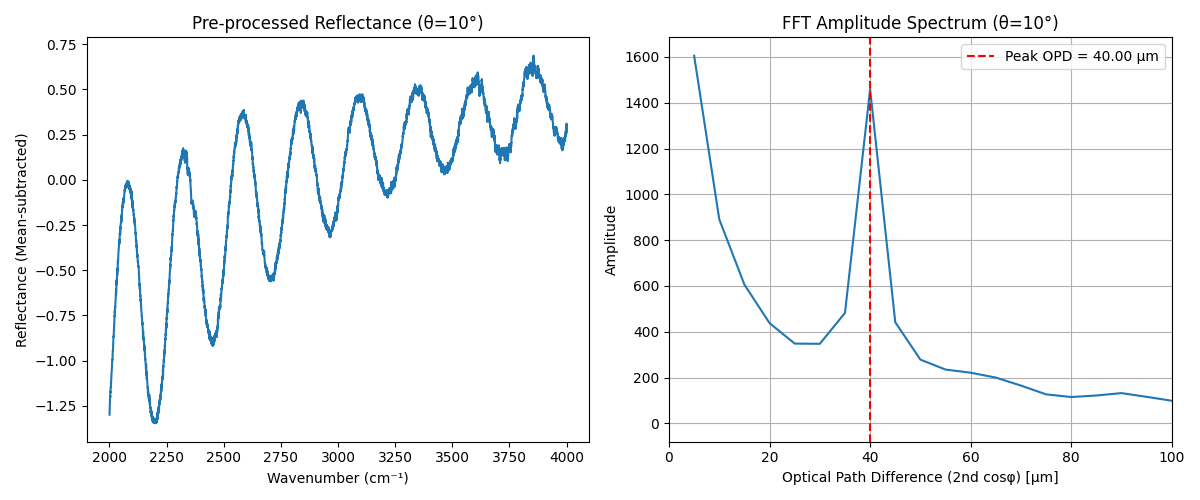
\includegraphics[width=0.9\textwidth]{fft_plot_10deg.png} % 请确保图片文件名为fft_plot_10deg.png
    % 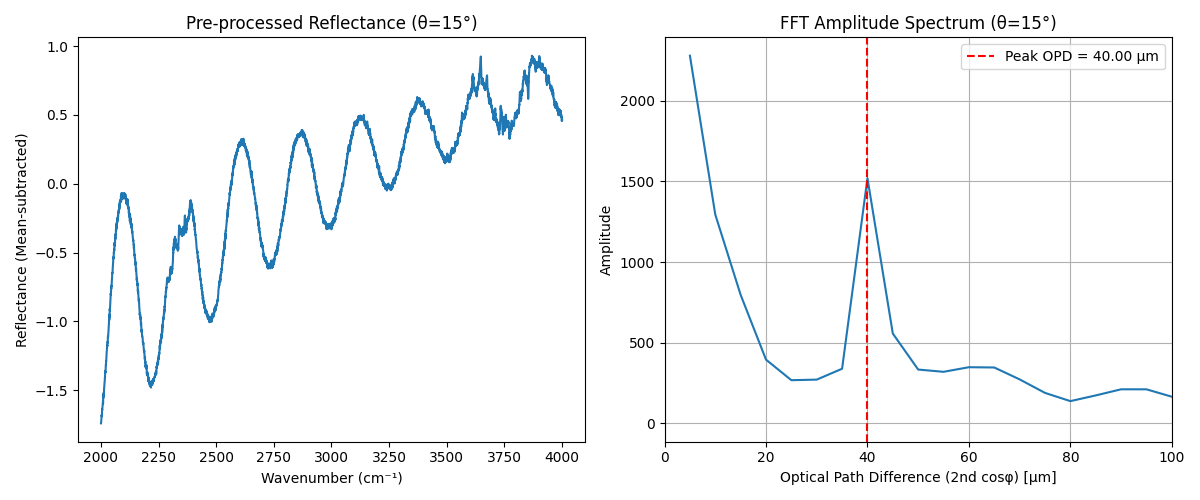
\includegraphics[width=0.9\textwidth]{fft_plot_15deg.png} % 请确保图片文件名为fft_plot_15deg.png
    % 先放置一个占位符
    \fbox{\parbox[c][12cm][c]{0.9\textwidth}{\centering FFT结果示意图占位符}}
    
    \caption{基于FFT方法对SiC样品光谱数据的分析(上:$\theta=10^\circ$,下:$\theta=15^\circ$)。左侧为预处理后的反射率信号,右侧为其FFT振幅谱。谱中的红色虚线标示出了光程差(OPD)主峰的位置。}
    \label{fig:fft_results}
\end{figure}

从图\ref{fig:fft_results}的右侧振幅谱中可以清晰地看到,在光程差(OPD)轴上出现了一个非常尖锐和独立的峰值,其位置分别对应了两个入射角下的光程差$L = 2nd\cos\phi$。这验证了FFT方法在提取核心周期性成分上的有效性。根据峰值位置计算出的外延层厚度结果,我们汇总于表\ref{tab:fft_results}中。

\begin{table}[htbp]
    \centering
    \caption{基于FFT方法消除多光束干涉影响后的SiC外延层厚度计算结果}
    \label{tab:fft_results}
    \begin{tabular}{ccc}
        \toprule
        附件                                & 入射角 $\theta$ ($^\circ$) & 计算厚度 $d$ ($\mu$m) \\
        \midrule
        1                                 & 10.0                    & 7.8611            \\
        2                                 & 15.0                    & 7.8836            \\
        \midrule
        \multicolumn{2}{c}{\textbf{平均厚度}} & \textbf{7.8724}                             \\
        \multicolumn{2}{c}{\textbf{相对误差}} & \textbf{0.29\%}                             \\
        \bottomrule
    \end{tabular}
\end{table}

\paragraph{结果分析与讨论}
从表\ref{tab:fft_results}可以看出,采用FFT方法对附件1和附件2的数据进行分析后,计算得到的两个厚度值分别为$7.8611\,\mu\text{m}$和$7.8836\,\mu\text{m}$。这两个值非常接近,它们之间的相对误差仅为$0.29\%$,计算公式如下:
$$ \varepsilon_d = \frac{|d_{10^\circ} - d_{15^\circ}|}{(d_{10^\circ} + d_{15^\circ})/2} = \frac{|7.8611 - 7.8836|}{(7.8611 + 7.8836)/2} \times 100\% \approx 0.29\% $$
该误差远小于5\%的常规容许范围,表明计算结果具有高度的自洽性和可靠性。

与我们在问题二中使用峰值间距法($\Delta\nu$法)得到的$2.28\%$的相对误差相比,当前$0.29\%$的误差有了显著的降低。这充分说明,多光束干涉效应确实对传统的峰值间距法造成了可观测的精度影响,而我们提出的FFT方法能够有效抑制这种影响以及其他噪声干扰,从而获得更加精确和稳健的厚度测量结果。

综上所述,我们认为通过FFT方法消除多光束干涉影响后,得到的碳化硅外延层厚度更为准确。我们取两个角度计算结果的平均值作为最终结论。

最终,我们确定该碳化硅外延层的厚度为 $\mathbf{7.87\,\mu m}$。

\end{document}

